\section{Method}
在本节中,我们详细阐述了DDPTransformer的实现过程。首先介绍DDPTransformer的整体架构,之后描述搭建网络过程中的细节以及loss function的选择。
\subsection{Overall Network Architecture}
从sinogram中重建出CT图像可表示为以下线性逆问题:
\begin{equation}
	\label{equation1}
	g = Af+\eta
\end{equation}
其中$g$是已经被测量出的singram(投影数据),$f$是其对应的高质量的CT图像,$A$是对成像系统进行建模的矩阵。$\eta$是噪声。事实上在2DCT重建任务中,$A$等价于平行光束成像几何的Radon变换,并且它是不可逆的。$\eta$大部分是Poisson noise。因此,this inverse problem is highly ill-posed。\par
我们的任务就是通过神经网络去拟合this inverse problem\ref{equation1}。网络的整体架构如图1(a)所示\ref{fig1},它由四个阶段组成,第一步对输入的sinogram使用双线性插值法来扩大探测器的数量,从而模拟出正常采样下得到的sinogram,但同时会造成sinogram过于平滑,噪声大等问题;第二步在Sinogram Domain SubNet中通过将DDPTransformer Block进行多次迭代来进行降噪和去平滑,另外由于sinogram图像是不具有局部特性的,所以我们通过Transformer来获取的全局信息的优势会更好的帮助我们重建出正常采样下的sinogram;第三步通过Filter BackProjection(FBP)算法进行空间域的变换,将sinogram转为CT图,但FBP算法会带来条纹伪影和噪声;最后在Image Domain SubNet中同样通过多个DDPTransformer Block进行多次迭代,通过LCL模块中的卷积操作,可以有效解决伪影和噪声,最终得到高质量的CT图像。在DDPTransformer的四个阶段中,阶段2的Sinogram Domain SubNet和阶段4的Image Domain SubNet是两个深度神经网络,所以我们要分别对其进行训练。图1(b)和图1(c)\ref{fig1}表示这两个子网络训练时的总体架构。\par
\begin{figure}
	\centering
	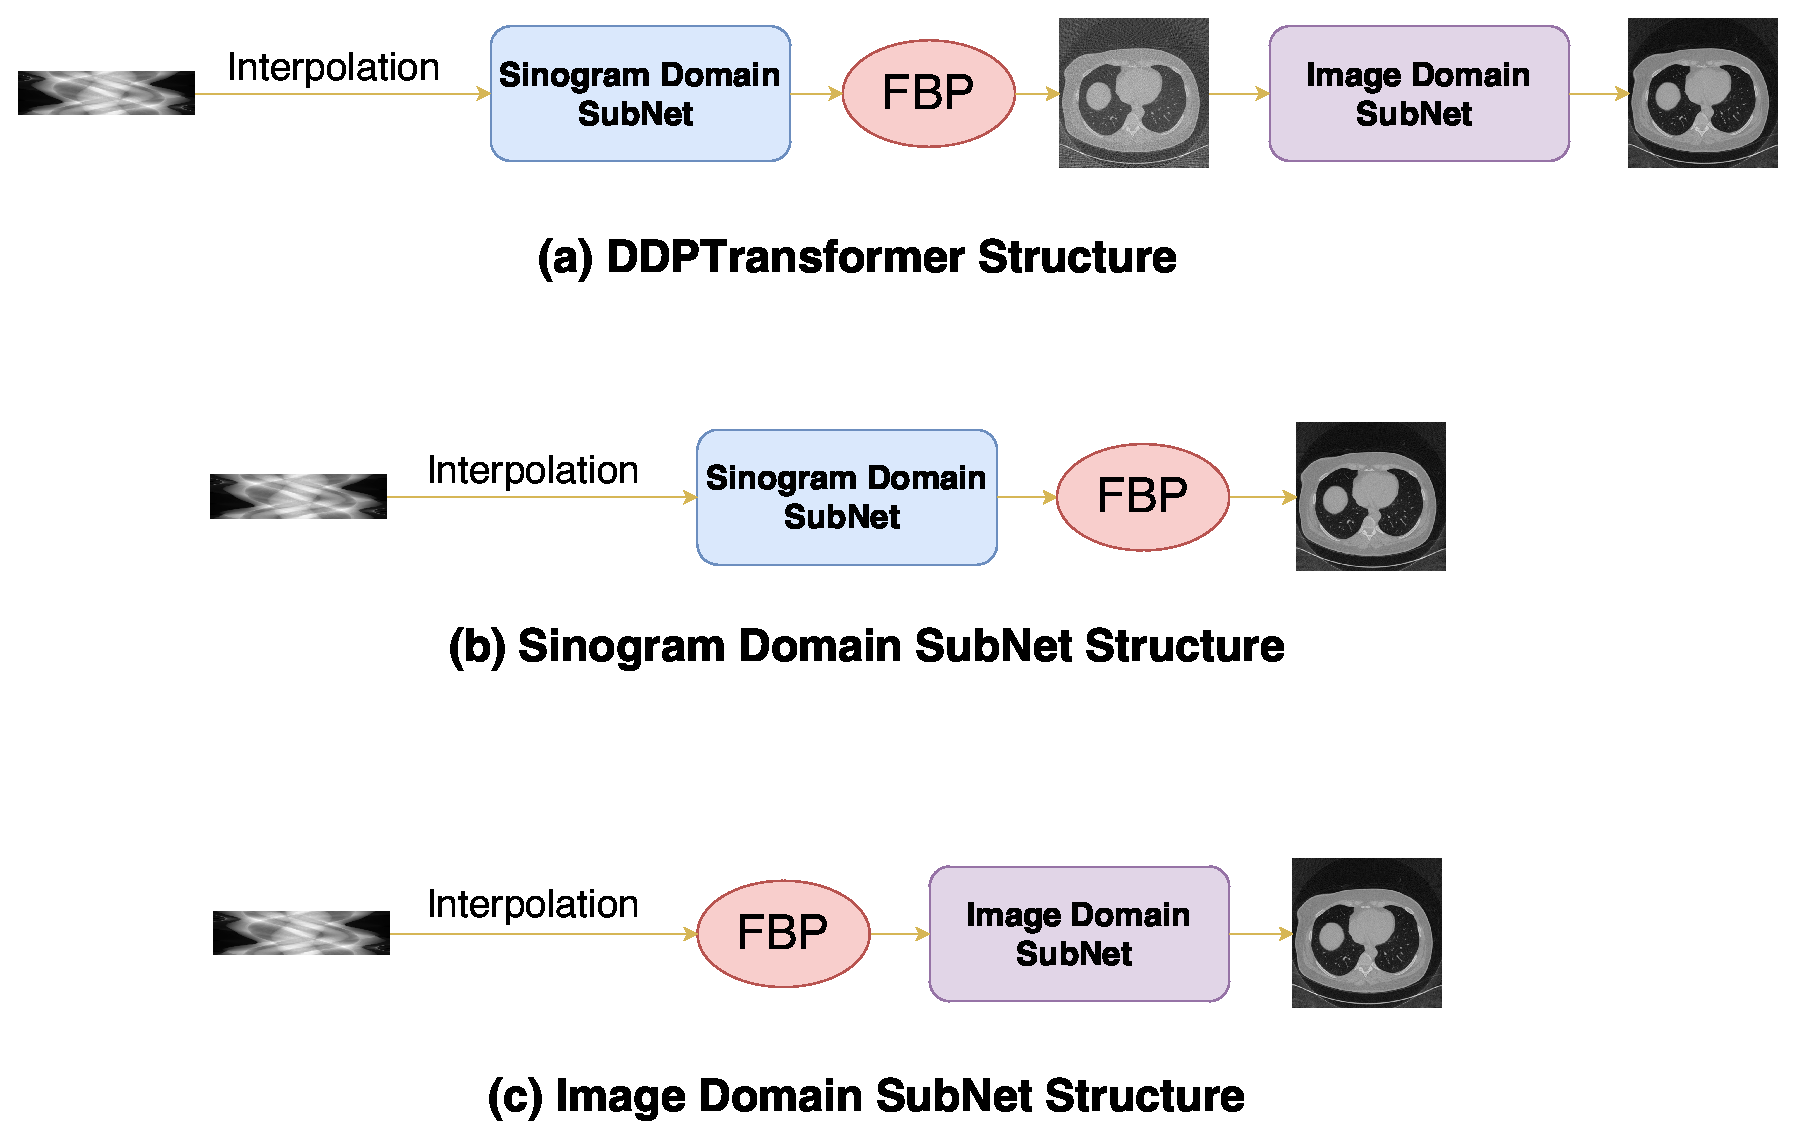
\includegraphics[height=8cm,width=12cm]{1.eps}
	\caption{The Overall structures of the DDPTransformer, Sinogram Domain SubNet
	 and Image Domain SubNet.}
	\label{fig1}
\end{figure}
在DDPTransformer中,Sinogram Domain SubNet 和 Image Domain SubNet 均由 DDPTransformer Block组成。所以在介绍两个SubNet之前,我们将详细说明DDPTransformer Block的结构和细节。
\subsection{DDPTransformer Block Design}

过去基于卷积的神经网络的特征提取是非常成功的,但卷积操作需要不断堆积卷积层来完成对图像从局部信息到全局信息的提取,不断堆积的卷积层慢慢地扩大了感受野直至覆盖整个图像,这会导致浅层的卷积层不会得到太多的全局信息。但transformer并不假定从局部信息开始,而是一开始就可以拿到全局信息,尽管训练难度更大一些(如所需要的数据集要更大些,以及所需要学习的参数量更多),但是一旦完成好训练,更早得到全局信息的优势会使得效果更好。我们提出的DDPTransformer Block流程如图2\ref{fig2}所示。\par
\begin{figure}
	\centering
	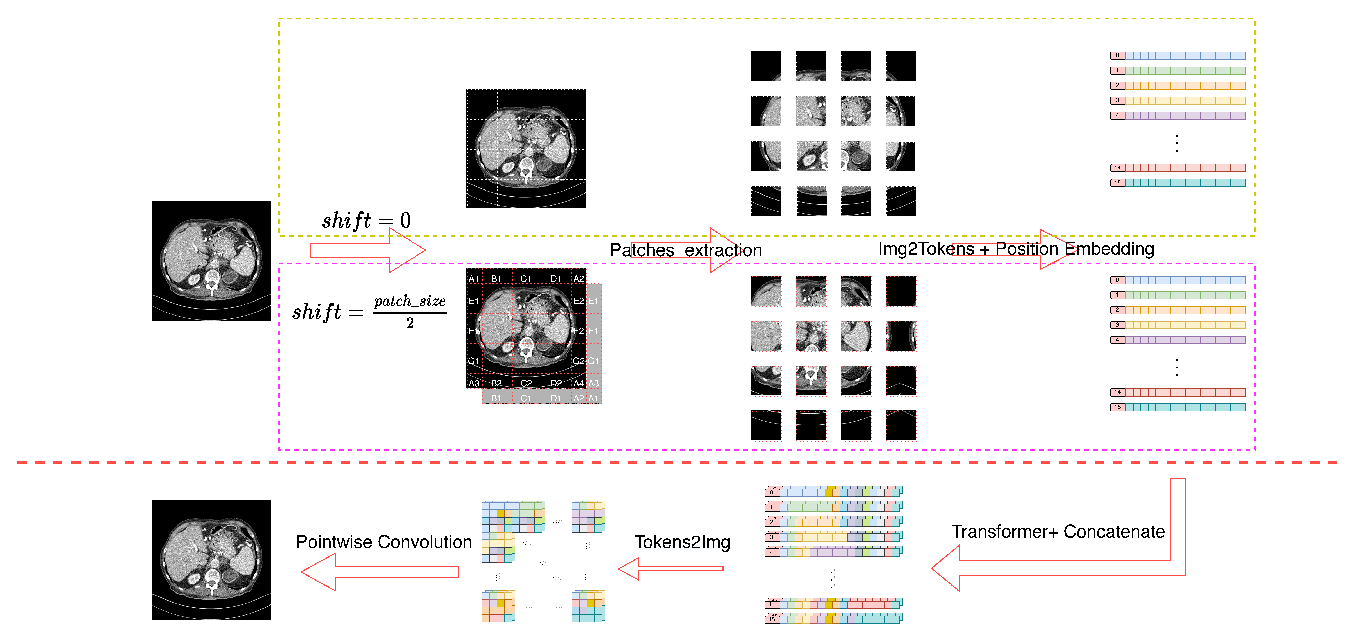
\includegraphics[height=8cm,width=18cm]{5.eps}
	\caption{DDPTransformer Block}
	\label{fig2}
\end{figure}
首先我们将输入图片$x \in \mathbb{R}^{H\times W \times C}$划分成相同大小的块(例如在图2中我们划分了16个Patch块),并根据两种不同的划分方案分别进行操作,where$(H,W)$是输入图片x的尺寸,$C$是通道。一种划分方案为$shift=0$(即图2黄色矩形框部分),即将输入图片划分成16宫格的形状$x_p \in \mathbb{R}^{\frac{H}{4}\times \frac{W}{4} \times 16C}$,之后因为标准Transformer接收的输入是一维序列,所以我们将每个$x_p$拉平为$x_d \in \mathbb{R}^{N \times 16C}$,where$N = \frac{H\times W}{16}$是每个$x_d$的长度。并参考Vision Transformer为每个序列加上Position embeddings以保留位置信息。另一种划分方案为$shift=\frac{patch\_size}{2}$(即图2紫色矩形框部分),首先将图片x沿右沿下平移$\frac{patch\_size}{2}$得到$x'$,即图2阴影部分。之后在$x'$上按照16宫格的形状在$x$上划分出尺寸不一的patch块$x_p$,并按照图中所示将部分$x_p$进行shift,如将$x$中的$A1$块移动到$x'$中的$A1$块,$x$中的$B1$块移动到$x'$中的$B1$块等。所有移动完成之后就可以得到尺寸一样的$x_p \in \mathbb{R}^{\frac{H}{4}\times \frac{W}{4} \times 16C}$,之后与第一种方案一样,将$x_p$拉平为$x_d \in \mathbb{R}^{N \times 16C}$并加上Position embeddings。\par

接着我们将两种方案得到的是一维序列分别输入到Transformer中。如图3(a)\ref{fig3}所示,Transformer由标准的多头自注意力(multi-head self attention (MSA))模块和Layer-Conv-Layer(LCL)模块组成(如图3(b)所示)。A layer
normalization(LN)\cite{ba2016layer}被用在每个模块之前,and a Skip Connection被用在每个模块之后。Transformer块的计算表示为:
\begin{equation}
\begin{aligned}
&\hat{x}_{d} = \mathrm{MSA}(\mathrm{LN}(x_{d-1}))+x_{d-1}   \\
&x_d= \mathrm{LCL}(\mathrm{LN}(\hat{x}_{d}))+\hat{x}_{d}\end{aligned}\end{equation}
其中$\hat{x}_{d-1} $和$x_d$分别为MSA模块和LCL模块的输出。下面,我们分别对MSA和LCL进行详细说明\par
\begin{figure}
	\centering
	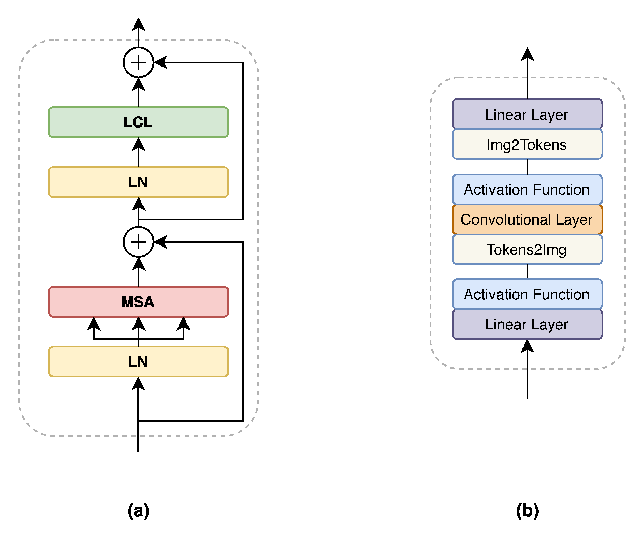
\includegraphics[height=8cm,width=10cm]{2v2.eps}
	\caption{Transformer and LCL structure.}
	\label{fig3}
\end{figure}

\textbf{Multi-head Self-Attention (MSA)}。我们将$x_{d-1} \in \mathbb{R}^{N \times 16C}$按Patches的个数将其分开并计算他们的自注意力,公式如下:
\begin{equation}
\begin{aligned}
&x_{d-1} = \{x^1_{d-1},x^2_{d-1},\cdots,x^n_{d-1}\}, \mathrm{n\;=\;number\;of\;Patch} \\
&y^i_{d-1} = Attention(x^i_{d-1}w^q,x^i_{d-1}w^k,x^i_{d-1}w^v), \mathrm{i=1,2,\cdots,n} \\
&\hat{x}_{d} = \{y^1_{d-1},y^2_{d-1},\cdots,y^n_{d-1}\},\mathrm{n\;=\;number\;of\;Patch} 
\end{aligned}
\end{equation}
其中$w^q$,$w^k$,$w^v$表示query,key and value的投影矩阵,Attention公式为:
\begin{equation}
\begin{aligned}
Attention(Q,K,V) = SoftMax(\frac{QK^T}{\sqrt{D}})V
\end{aligned}\end{equation}
其中D表示query/key的维数。上述过程为计算一个头的自注意力,假设头数为$k$,即上述公式重复$k$次,得到$\{\hat{x}^1_{d},\hat{x}^2_{d},\cdots,\hat{x}^k_{d}\}$,并将其Concat得到最终MSA的输出$\hat{x}_{d}$。而为了保证参数的计算和数量不变,需要将D缩小k倍。\par
\textbf{Layer-Conv-Layer(LCL)}。MSA模块注重于融合更多的全局信息,但是对于如何学习这些信息的能力却不足,所以我们通过LCL模块来弥补学习能力。由于MSA的输出是1-D序列,所以大多数都是通过MLP来进行学习。虽然我们加了位置信息来拟补2-D拉平为1-D导致降维带来的部分特征丢失,但我们认为更好的解决方案是直接在2-D上进行学习。所以在MLP中加入一个卷积操作。整个流程如图3(b)\ref{fig3}所示,我们首先对$\hat{x}_{d}$用Linear Layer并使用激活函数,之后reshape为2-D并使用卷积和激活函数进行学习。之后在拉平回1-D并再次用Linear Layer得到输出$x_d$。\par

两种方案($shift=0$和$shift=\frac{patch\_size}{2}$)分别使用Transformer之后,我们将其输出Concat。使用两种方案是为了互相弥补patch块的边缘信息,所以我们选择将其再次reshape为2-D而不是直接在1-D上进行互补。最后通过Point-Wise Convolution\cite{2017Xception}得到输出。\par

\subsection{Sinogram Domain SubNet}
如图4紫色虚线框\ref{fig4v2}所示,Sinogram Domain SubNet采用流式架构,他由3部分组成。首先将经过插值之后的 sinogram image 通过Input Projection扩大通道数并将每个通道进行Flatten操作,变成1-D的token。其次我们使用$n$个DDPTransformer Block组成Sinogram Domain SubNet的backbone,$n$的值我们会通过实验选出最优值,并且使用skip connection使模型更容易拟合。最后通过Output Projection将1-D的token输出得到重建之后的Sinogram Domain。在训练Sinogram Domain SubNet时,我们使用 the mean square error (MSE) 作为我们的损失函数:
\begin{equation}
\begin{aligned}MSE_{Loss}(X^{'},Y) = \mid X^{'}-Y\mid^{2}\end{aligned}\end{equation}
其中$X^{'}$表示经过模型计算并通过FBP算法得到的CT图,$Y$是对应的高质量的CT图(label)。\par
\begin{figure}
	\centering
	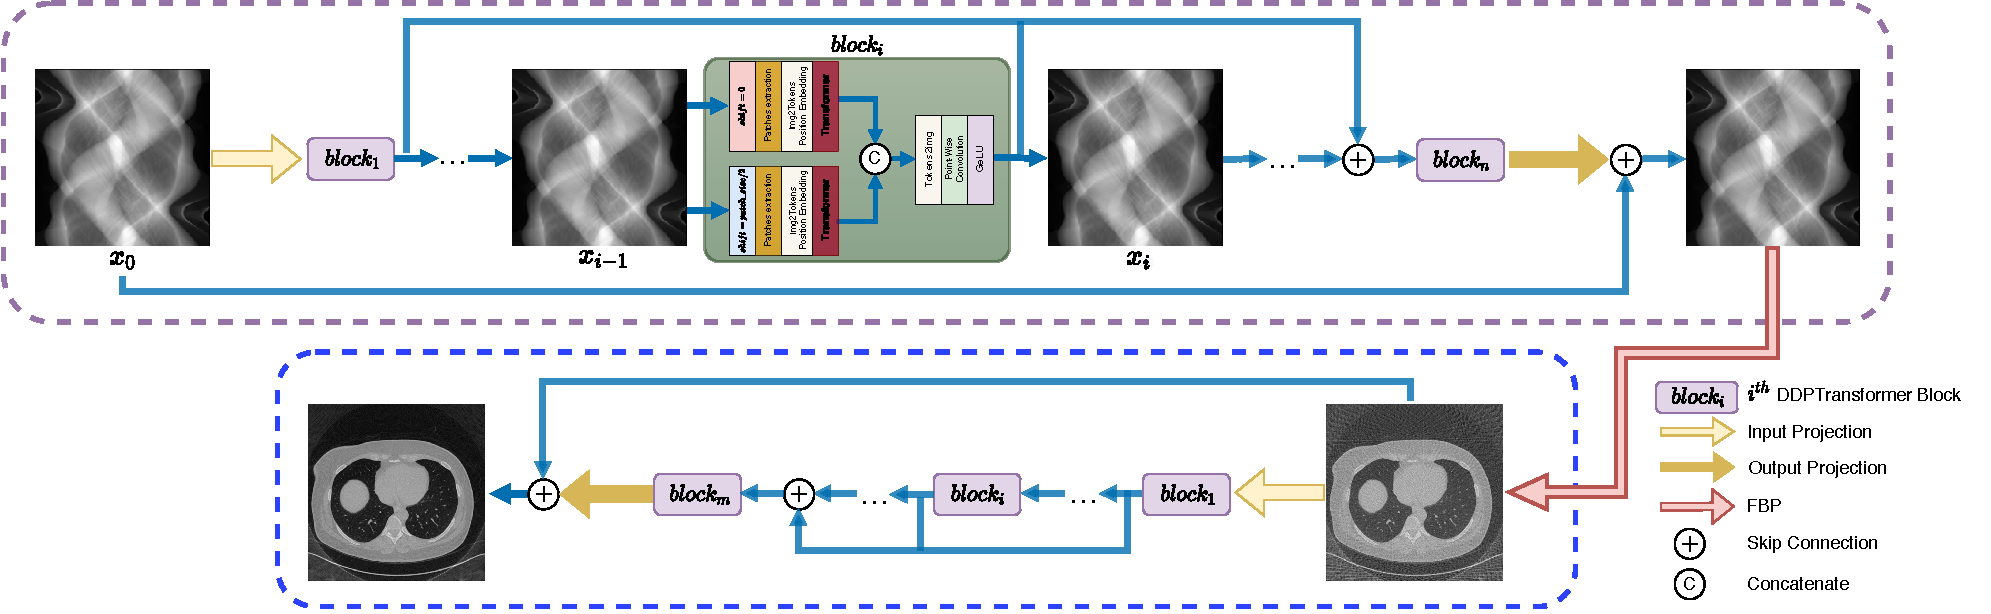
\includegraphics[height=5.5cm,width=18cm]{4v2.eps}
	\caption{DDPTransformer,紫色虚线框为Sinogram Domain SubNet,蓝色虚线框为Image Domain SubNet。}
	\label{fig4v2}
\end{figure}
\subsection{Image Domain SubNet}
由于FBP重构的CT图像受到条纹伪影和噪声的影响而退化,所以我们通过Image Domain SubNet来重建出高质量的CT图。如图4蓝色虚线框所示,Image Domain SubNet整体架构和Sinogram Domain SubNet类似。不同的是我们选用了$m$个DDPTransformer Block模块,同样$m$的值会通过实验得出。为了加快模型的收敛速度以及使得模型的performance更好,我们使用了Charbonnier Loss\cite{2017Fast}作为损失函数:
\begin{equation}\begin{aligned}
Charbonnier_{Loss}(X^{'},Y) = \sqrt{(X^{'}-Y)^{2} + \epsilon^{2}} \end{aligned}
\end{equation}
其中$X^{'}$表示我们最终重建得到的CT图,$Y$是对应的高质量的CT图(label)。$\epsilon$的值为常量$10^{-3}$。\par